% !TeX root = ../../main.tex
% Add the above to each chapter to make compiling the PDF easier in some editors.

\chapter{Background and Foundations}\label{chapter:Background and Foundations}

This chapter represent the basic concepts used throughout our work. First, brief introduction to the reinforcement learning field. Second, Markov Decision Processes (MDPs), the standard mathematical formalism framework for reinforcement learning will be introduced with some basic principles of reinforcement learning. Then, We will discuss the Value functions and Policy Gradient with the focus on Q-Learning. Next we will discuss the methods used and differentiate between them. After that, we conclude with  the use of deep learning with reinforcement learning and the different Deep Reinforcement Learning Algorithms. Finally, we  discuss the challenges and limitation in Reinforcement Learning.

\section{Reinforcement Learning}
Reinforcement Learning (RL) is a machine learning approach to teach agent how to solve tasks through trail and error interaction with a dynamic, unknown environment by maximizing a cumulative reward. The main characters of RL are the \textbf{Agent} and the \textbf{Environment}. The environment is the world where the agent lives and interacts with. for every interaction, the agent observe the state of the world and based on that takes an action. The environment changes accordingly to the agent's actions and it might also changes on its own. The typical interaction loop between agent and environment is illustrated in Figure \ref{fig:Agent_Env}

\begin{figure}
  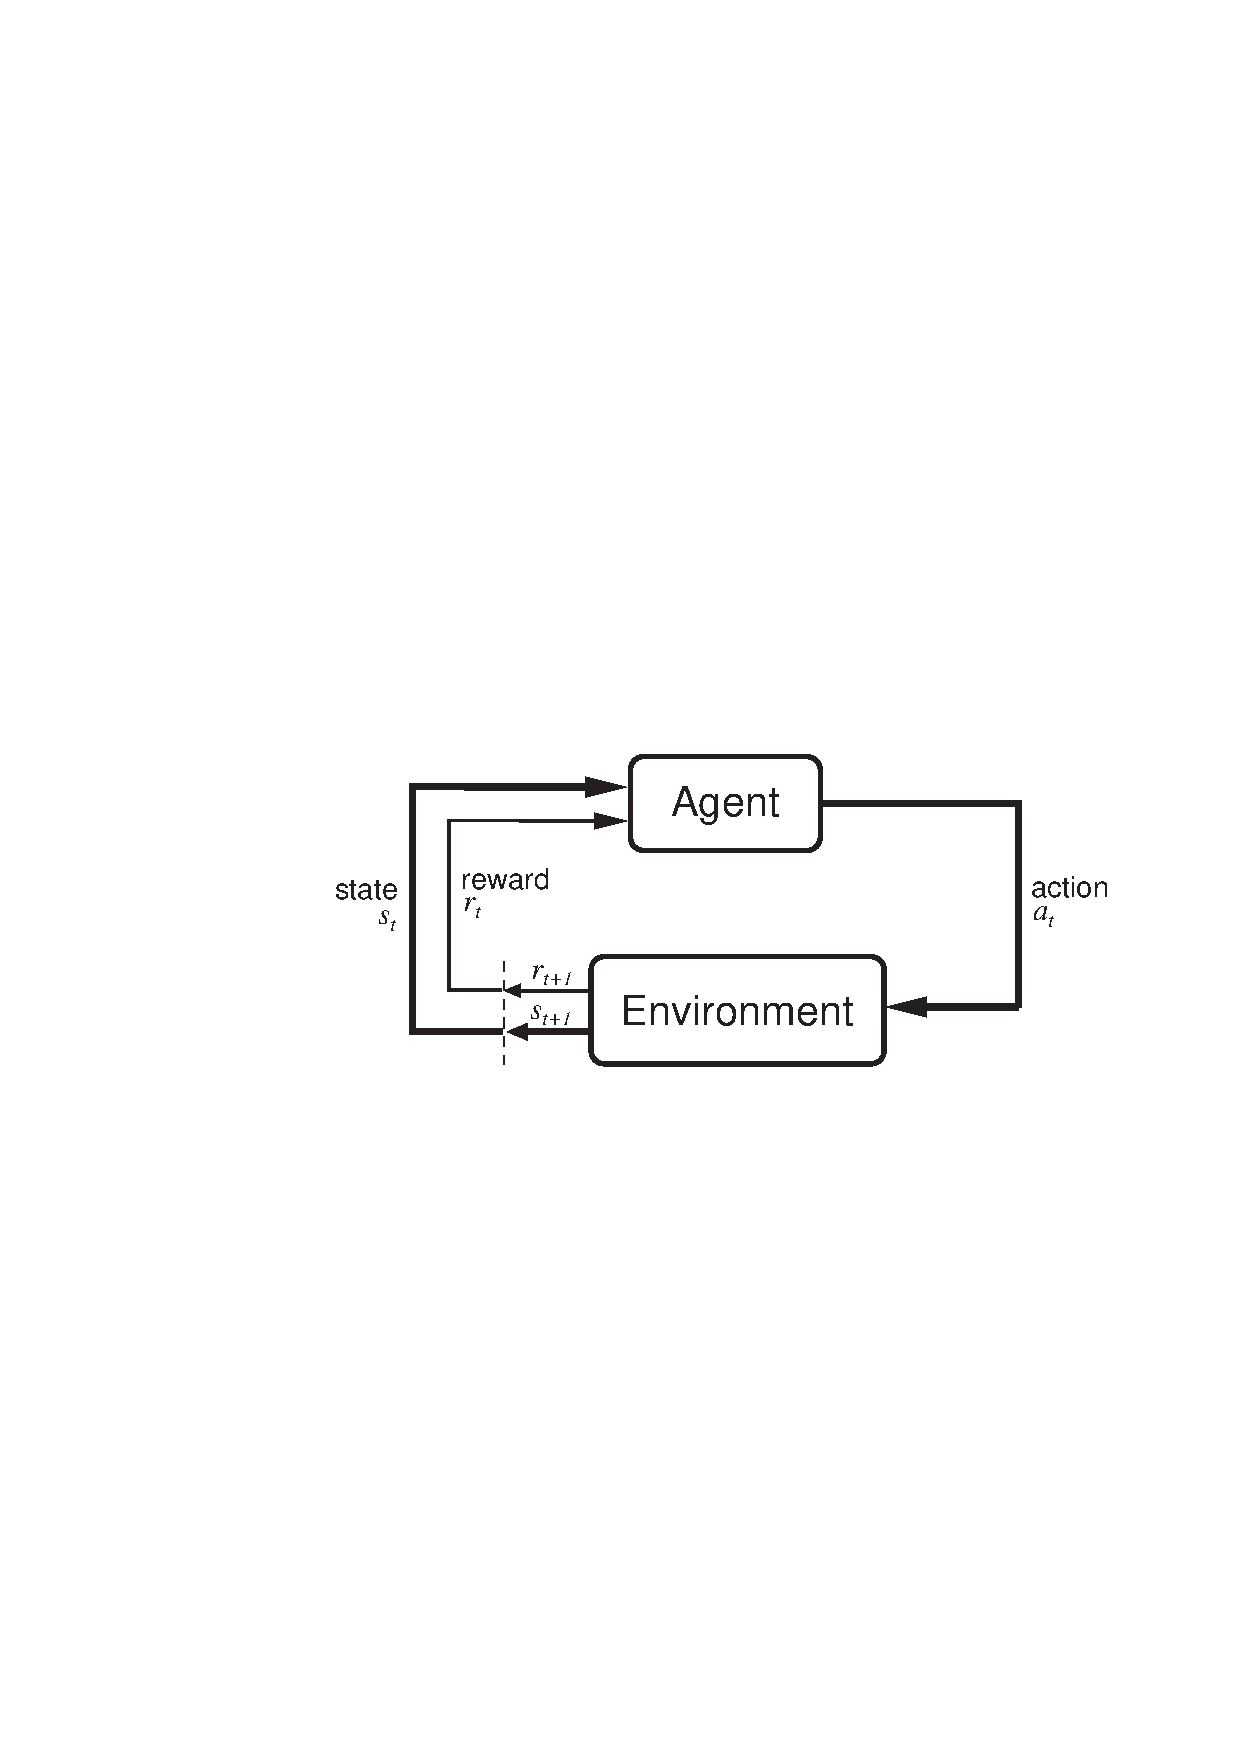
\includegraphics[width=\linewidth]{figures/Agent-Env.jpg}
%   \caption{Reinforcement Learning interaction loop. The agent takes an action at a\textsubscript{t} state s\textsubscript{t}. The environment then responds with the corresponding reward r\textsubscript{t+1} and the new state s\textsubscript{t+1}, which are fed back to the agent [\citetitle{sutton2018reinforcement}]}
  \caption{Reinforcement Learning interaction loop. [\citetitle{sutton2018reinforcement}]}
  \label{fig:Agent_Env}
\end{figure}

\subsection{Markov Decision Process}
\subsection{Value Functions}
\subsection{Policy Gradient}
\subsection{Q-Learning}
\subsection{Reinforcement learning methods}
    \subsubsection{Model-free}
    \subsubsection{Model-based}
\subsection{Limitations of RL in practice}

\section{Deep Reinforcement Learning}
\subsection{Overview}
\subsection{Deep Q Network}
\subsection{Deep Deterministic Policy Gradient}
\subsection{Proximal Policy Optimization}
\subsection{Asynchronous Advanced Actor Critic (\textbf{A3C})}

% \section{Literature Review}

\section{Challenges in Reinforcement Learning}